\documentclass[margin=0.5mm]{standalone}
\usepackage{pgfplots}
\usetikzlibrary{pgfplots.groupplots}
\pgfplotsset{compat=1.7}

\begin{document}
	\thispagestyle{empty}
		\centering
		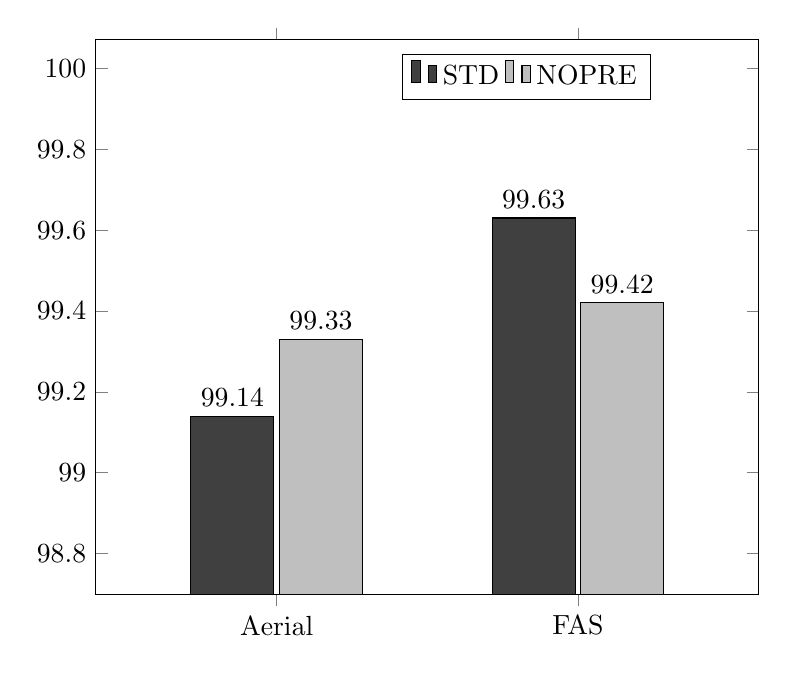
\begin{tikzpicture}
		\begin{axis}[
			width=10cm,
				enlarge x limits=0.6,
				enlarge y limits=0.9,
					ybar,
					legend style={at={(0.65,0.975)},
					anchor=north,legend columns=-1},
					symbolic x coords={Aerial,FAS},
					xtick=data,
				  nodes near coords={\pgfmathprintnumber[fixed zerofill, precision=2]{\pgfplotspointmeta}},
					nodes near coords align={vertical},
					bar width=30pt,
					style={font=\normalsize},
					ytick={98.0,98.2,...,100.1}
		]
		%						STD		NPRE	
		%			Aerial
		%				Clean	99.89	99.62	
		%				Noisy   99.14	99.33
		
		%			FAS		
		%				Clean	100 	100 	
		%				Noisy   99.63	99.42	
		
		
		\addplot [color=black,fill=darkgray] coordinates {(Aerial,99.14) (FAS,99.63)  };
		\addplot [color=black,fill=lightgray] coordinates {(Aerial,99.33) (FAS,99.42) };		
		
		\legend{STD,NOPRE,NOPRELP}
		\end{axis}
		\end{tikzpicture}
		
		%\vspace{-0.7cm}
		%\caption{Left: the pitch distribution for the 10 male speakers. Right: the active speech level for the 20 speakers.}\label{fig:pitch}
		%\vspace{-0.5cm}
\end{document}